\documentclass[12pt]{report}
\usepackage[utf8]{inputenc}
\usepackage{graphicx}
\begin{document}
\begin{center}
    {\Large How does the time it takes a ball to roll down a slope depend on the distance it travels?}
    
    \vspace{1cm}
    {\large Jason Wells, Kevin Qiao, Stephen Okita and Terri Tai}
    \center{{\large Experiment performed: 20/10/2021}}
    {\large Reprt submitted: 26/10/2021}
    \vspace{2cm}
    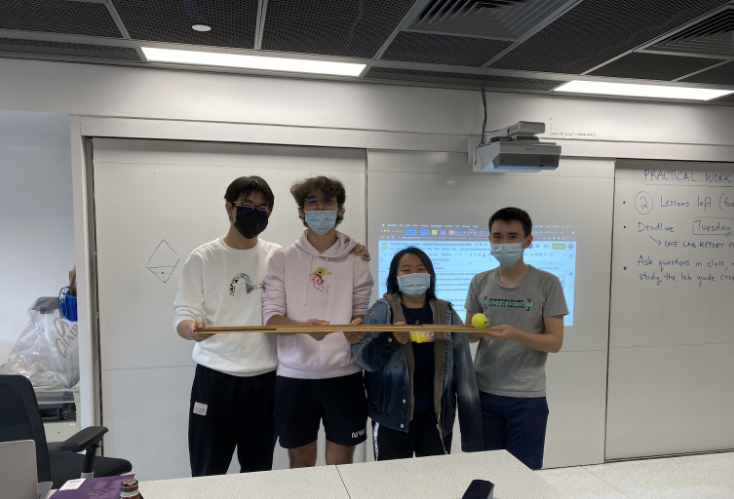
\includegraphics[width=\textwidth]{Img.png}

\end{center}
\tableofcontents{document}
\section{Introduction}


\[ y = \sqrt{\frac{2x}{-9.8(\sin(5.17))-0.14\cos(5.17)}}\]

\end{document}\